\documentclass{article}
\usepackage[utf8]{inputenc}
\usepackage{cite}
\usepackage{graphicx}
\usepackage{algorithm}
\usepackage{algorithmic}
\title{214712239-Huan Yang}
\author{Huan Yang}
\date{November 2021}

\begin{document}

\maketitle


\section{Latex Class 1 - How to add references ?}

\subparagraph{ResNet \cite{DBLP:journals/corr/HeZRS15}} 
% \subparagraph{Wille1982 \cite{Wille1982} }


\section{Latex Class 2 - How to add a table ?}
\paragraph{Table~\ref{tab:my_label} shows the people who are awesome.}
\begin{table}[htbp]\large

    \centering
    \begin{tabular}{|c c c|}
        \hline
        \multicolumn{3}{|c|}{Messege}\\
        \hline
        name & class & id \\ 
        \hline
        Huan Yang & 1 & 001 \\
        Shiye Tabf & 2 & 002 \\
        Mazi Zhang & 3 & 003 \\
        \hline

    \end{tabular}
     \caption{Test Table}
    \label{tab:my_label}
\end{table}

\section{Latex Class 3 - How to add a figure ?}
\paragraph{I also like dogs Figure~\ref{fig:dog}. }
\paragraph{I like to travel, I came to the mountain of life Figure~\ref{fig:nature}. }



\begin{figure}[h]
\centering

\includegraphics[scale=0.25]{dog.jpg}
\caption{this is a dog.}
\label{fig:dog}
\end{figure}

\begin{figure}[h]
\centering
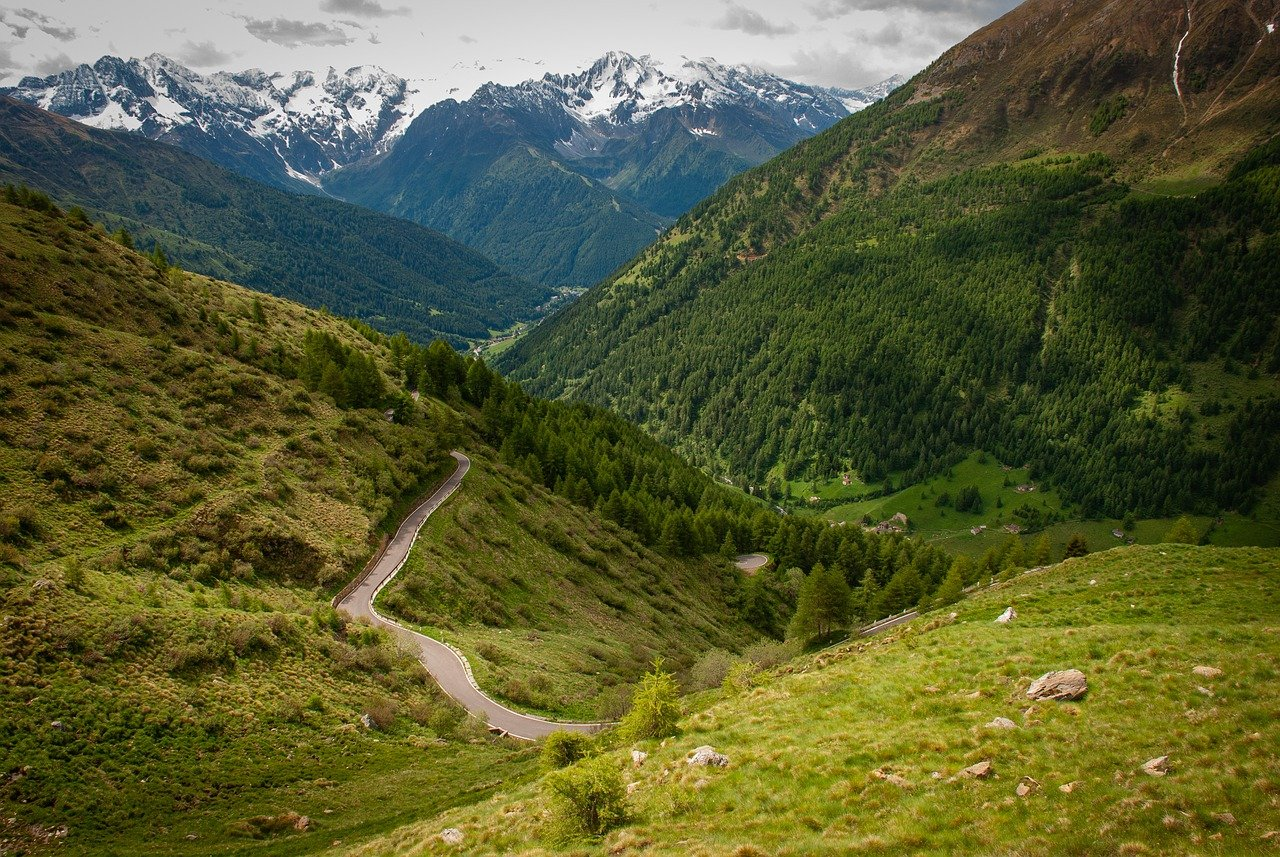
\includegraphics[scale=0.25]{fig1.jpg}
\caption{this is the mountain of life.}
\label{fig:nature}
\end{figure}

\section{Latex Class 4 - How to add a algorithm ?}
\begin{algorithm} 
	\caption{Calculate $y = x^n$} 
	\label{alg3} 
	\renewcommand{\algorithmicrequire}{\textbf{Input:}}
	\renewcommand{\algorithmicensure}{\textbf{Output:}}
	\caption{Bayesian Personalized Ranking Based Latent Feature Embedding Model}
	\label{alg:1}
	\begin{algorithmic}[1]
		\REQUIRE $A$,$B$,$C$
		\ENSURE $(A+B)\times C$
		\STATE SET $D=0$ as return value
 		\FOR {$i$ in $C$}
 		\STATE Update $D=D+A\times B$
 		\ENDFOR
		\STATE \textbf{return} $D$
	\end{algorithmic}  
\end{algorithm}


\bibliographystyle{plain}
\bibliography{ref}
\end{document}
